In order to understand the power and the importance of Feedforward Networks, we first need to understand
the limitations of linear models. Linear models are a class of models that make predictions 
based on a linear combination of the input features. They are simple and efficient, but they 
have limitations in capturing complex relationships in data. In Table \ref{tab:linear_models}, we 
summarize the main types of linear models, their output functions, output ranges, and loss functions.
\begin{table}[htbp]
  \centering
  \small
  \begin{tabular}{lllll}
    \toprule
    \textbf{Task} & \textbf{Score} & \textbf{Output function} & \textbf{Output range} & \textbf{Loss} \\
    \midrule
    Regression & $z = \mathbf{w}^{\top}\mathbf{x} + b$ & identity: $\hat{y} = z$ & $\mathbb{R}$ & $(\hat{y} - y)^2$ \\
    Binary (hinge) & $z = \mathbf{w}^{\top}\mathbf{x} + b$ & $\hat{y} = \text{sign}(z)$ & $\{-1, +1\}$ & $\max(0, 1 - y z)$ \\
    Binary (logistic) & $z = \mathbf{w}^{\top}\mathbf{x} + b$ & $\hat{y} = \sigma(z)$ & $(0, 1)$ & $-y \log \hat{y} - (1 - y) \log(1 - \hat{y})$ \\
    Multi-class & $z = \mathbf{W}^{\top}\mathbf{x} + \mathbf{b}$ & $\hat{\mathbf{y}} = \text{softmax}(\mathbf{z})$ & probability vectors & $-\log \hat{y}_y$ \\
    \bottomrule
  \end{tabular}
    \caption{Models with a Linear Score}
    \label{tab:linear_models}
\end{table}
\section{Score Function of Linear Models}
Every task solved with a linear model relies on a score function that computes a linear combination 
of the input features. The score (often denoted as $z$ or referred to as \textit{logits} in 
classification) represents the initial, raw evidence or confidence calculated by the model before
any final mapping. For regression and binary classification tasks, given a single input vector 
$\mathbf{x} \in \mathbb{R}^d$, the score is a scalar computed as a weighted sum plus a bias:
\begin{equation}
    z = \mathbf{w}^{\top}\mathbf{x} + b
\end{equation}
Geometrically, this score defines a single hyperplane in the input space that serves as the decision 
boundary ($z = 0$) or predicts a continuous value (in the case of regression). 
\newline
For multi-class tasks with $k$ classes, the model 
computes a vector of scores rather than a single scalar. Using matrix notation for a weight 
matrix $\mathbf{W}$ and a bias vector $\mathbf{b}$:
\begin{equation}
    \mathbf{z} = \mathbf{W}^{\top}\mathbf{x} + \mathbf{b}
\end{equation}
In this multi-class setting, the model evaluates multiple scores simultaneously, where the boundaries 
between classes are formed where individual score components equate ($z_i = z_j$).

\section{Output And Loss Function of Linear Models}
The output and loss functions are different for each task, the first maps the raw score to the final 
prediction and the second measures the error between the prediction $\hat{y}$ and the true target $y$
in order to be able to update the model parameters. 

\subsection{Regression}
In regression, the output function is the identity function, meaning the raw score is used directly 
as the prediction:
\begin{equation}
    \hat{y} = z
\end{equation}
So the output range is the entire set of real numbers ($\mathbb{R}$). In Fig. \ref{fig:linear_regression_2d}
there is an example of a linear regression in 2d (one feature).
\begin{figure}[htbp]
    \centering
    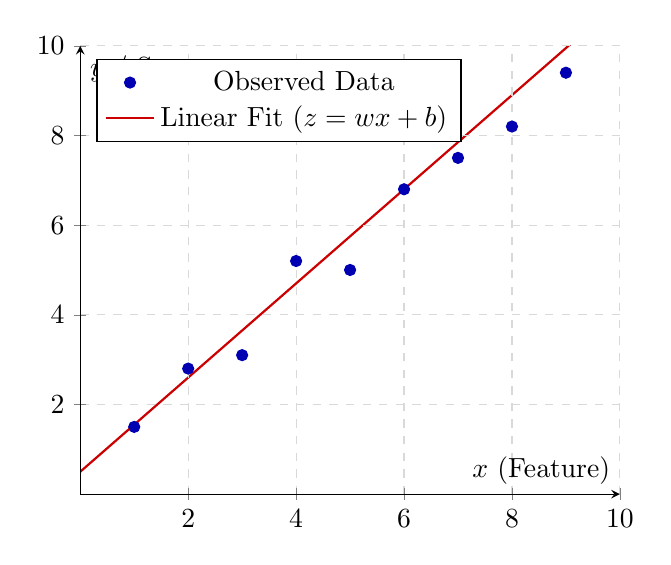
\begin{tikzpicture}
        \begin{axis}[
            xlabel={$x$ (Feature)},
            ylabel={$y$ / Score $z$},
            xmin=0, xmax=10,
            ymin=0, ymax=10,
            axis lines=center,
            axis on top=true,
            grid=major,
            grid style={dashed, gray!30},
            legend pos=north west
        ]
            % Punti del dataset (osservazioni reali)
            \addplot[only marks, mark=*, blue!70!black] coordinates {
                (1, 1.5) (2, 2.8) (3, 3.1) (4, 5.2) (5, 5.0) 
                (6, 6.8) (7, 7.5) (8, 8.2) (9, 9.4)
            };
            
            % Retta di regressione (il modello lineare: z = w*x + b)
            \addplot[domain=0:10, red!80!black, thick] {1.05 * x + 0.5};
            
            \legend{Observed Data, Linear Fit ($z = wx + b$)}
        \end{axis}
    \end{tikzpicture}
    \caption{Geometric representation of 2D linear regression.}
    \label{fig:linear_regression_2d}
\end{figure}
\newline
The loss function for regression is the \textbf{Squared Error}:
\begin{equation}
    l(\hat{y}, y) = (\hat{y} - y)^2
\end{equation}
that means that the loss grows quadratically with the error, which can be sensitive to outliers.
\newline
so it's often used the \textbf{Absolute Error}:
\begin{equation}
    l(\hat{y}, y) = |\hat{y} - y|
\end{equation}
that grows only linearly.
\newline
In figure \ref{fig:loss_function_comparison} we can see a comparison between the two loss functions
if we take tre example ($\hat{y}$,y): (3,5;3)(2;3)(5;3). As we can se the squared error is geometrically
a parabola and the absolute error is a V shape.
\begin{figure}[H]
    \centering
    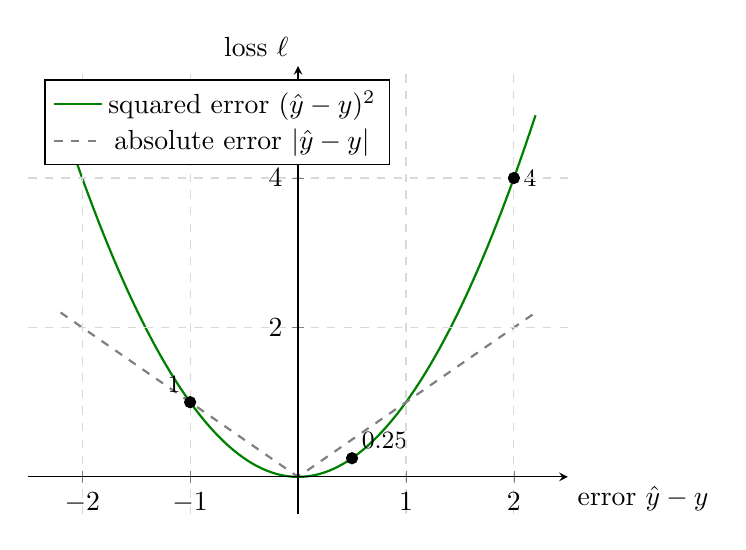
\begin{tikzpicture}
        \begin{axis}[
            xlabel={error $\hat{y} - y$},
            ylabel={loss $\ell$},
            xmin=-2.5, xmax=2.5,
            ymin=-0.5, ymax=5.5,
            axis lines=center,
            axis on top=true,
            grid=major,
            grid style={dashed, gray!30},
            legend pos=north west,
            every axis x label/.style={at={(current axis.right of origin)},anchor=north west},
            every axis y label/.style={at={(current axis.above origin)},anchor=south east}
        ]
            % Curva della squared error loss (parabola): (y_hat - y)^2
            \addplot[domain=-2.2:2.2, samples=100, green!50!black, thick] {x^2};
            \addlegendentry{squared error $(\hat{y} - y)^2$}

            % Linea della absolute error loss (valore assoluto): |y_hat - y|
            \addplot[domain=-2.2:2.2, samples=100, gray, dashed, thick] {abs(x)};
            \addlegendentry{absolute error $|\hat{y} - y|$}

            % Punti specifici evidenziati nella tabella d'esempio
            \addplot[only marks, mark=*, black] coordinates {
                (0.5, 0.25)
                (-1.0, 1.0)
                (2.0, 4.0)
            };

            % Etichette dei valori di loss in corrispondenza dei punti
            \node[above right] at (axis cs:0.5, 0.25) {\small $0.25$};
            \node[above left] at (axis cs:-1.0, 1.0) {\small $1$};
            \node[right] at (axis cs:2.0, 4.0) {\small $4$};

        \end{axis}
    \end{tikzpicture}
    \caption{Comparison between squared error loss and absolute error loss for linear regression.}
    \label{fig:loss_function_comparison}
\end{figure}

\subsection{Binary Classification (Hinge)}
In this type of classification task (e.g Support Vector Machines), the output function is the sign 
function, which maps the raw score to either -1 or +1:
\begin{equation}
    \hat{y} = \text{sign}(z)
\end{equation}
where 
\[
\text{sign}(z) = \begin{cases}
    +1 & \text{if } z > 0 \\
    0 & \text{if } z = 0 \\
    -1 & \text{if } z < 0
\end{cases}
\]
\begin{figure}[H]
    \centering
    \begin{tikzpicture}
        \begin{axis}[
            xlabel={Score $z$},
            ylabel={Output $\hat{y}$},
            xmin=-3.0, xmax=3.0,
            ymin=-1.5, ymax=1.5,
            axis lines=center,
            axis on top=true,
            grid=major,
            grid style={dashed, gray!30},
            ytick={-1, 1},
            yticklabels={$-1$, $+1$},
            every axis x label/.style={at={(current axis.right of origin)},anchor=north west},
            every axis y label/.style={at={(current axis.above origin)},anchor=south east}
        ]
            % Ramo negativo: y = -1 per z < 0
            \addplot[domain=-3.0:0, samples=2, blue!70!black, thick] {-1};
            
            % Ramo positivo: y = +1 per z > 0
            \addplot[domain=0:3.0, samples=2, blue!70!black, thick] {1};

            % Punti di discontinuità nell'origine (z = 0)
            \addplot[only marks, mark=*, blue!70!black] coordinates {(0,1)};
            \addplot[only marks, mark=o, blue!70!black] coordinates {(0,-1)};

        \end{axis}
    \end{tikzpicture}
    \caption{Output function for SVM / Hinge loss classification: $\hat{y} = \text{sign}(z)$.}
    \label{fig:svm_output_function}
\end{figure}
The loss function for binary classification with hinge loss is defined as:
\begin{equation}
    l(\hat{y}, y) = \max(0, 1 - yz)
\end{equation}
This function identifies three cases:
\begin{enumerate}
    \item $yz < 0$: the prediction is wrong and the loss grows linearly.
    \item $0 \leq yz < 1$: the prediction is correct, but it is too close to the decision boundary.
    \item $yz \geq 1$: the prediction is correct and sufficiently far from the boundary, so the loss is zero.
\end{enumerate}
In the $2^nd$ case we have a value of z equal to 0 or close to it, so a very small variation (i.e. a noise)
could lead to the opposite classification, so the loss isn't 0 even if the prediction is correct.
This is the geometric intuition behind margin maximization: the model is penalized only when the prediction is either wrong or not confident enough.
In Fig \ref{fig:hinge_loss} there is a raffiguration of what written above if we consider three cases of (y;z): (+1;3)(+1;0,4)(-1;2).
\begin{figure}[H]
    \centering
    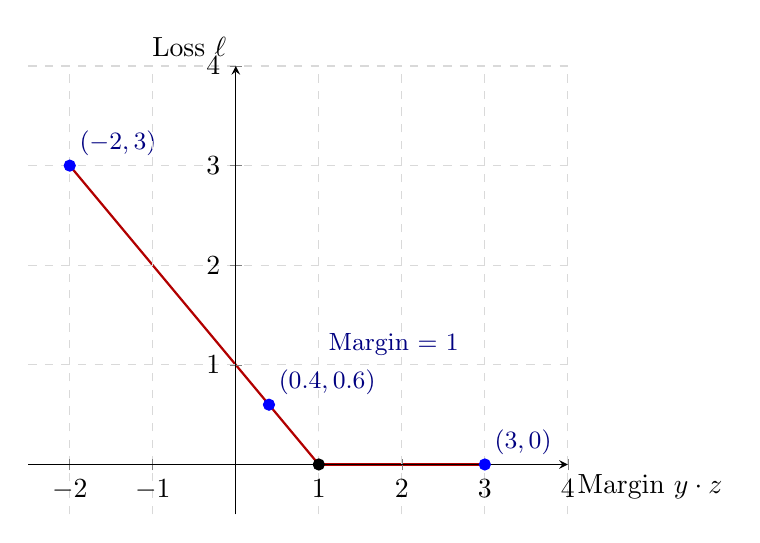
\begin{tikzpicture}
        \begin{axis}[
            xlabel={Margin $y \cdot z$},
            ylabel={Loss $\ell$},
            xmin=-2.5, xmax=4,
            ymin=-0.5, ymax=4,
            axis lines=center,
            axis on top=true,
            grid=major,
            grid style={dashed, gray!30},
            every axis x label/.style={at={(current axis.right of origin)},anchor=north west},
            every axis y label/.style={at={(current axis.above origin)},anchor=south east}
        ]
            % Funzione Hinge Loss: max(0, 1 - x)
            \addplot[domain=-2.0:1.0, samples=50, red!70!black, thick] {1 - x};
            \addplot[domain=1.0:3.0, samples=50, red!70!black, thick] {0};

            % Linea verticale di confine del margine (1.0)
            \draw[dashed, blue!50!black] (axis cs:1.0,0) -- (axis cs:1.0,1) node[above right, font=\small] {Margin = 1};

            % Punto di flesso originario a (1,0)
            \addplot[only marks, mark=*, black] coordinates {(1.0, 0.0)};

            % Punti degli esempi aggiunti (da[cite: 1])
            \addplot[only marks, mark=*, blue] coordinates {
                (3.0, 0.0)
                (0.4, 0.6)
                (-2.0, 3.0)
            };

            % Etichette opzionali per i punti
            \node[above right, blue!50!black, font=\small] at (axis cs:3.0, 0.0) {$(3, 0)$};
            \node[above right, blue!50!black, font=\small] at (axis cs:0.4, 0.6) {$(0.4, 0.6)$};
            \node[above right, blue!50!black, font=\small] at (axis cs:-2.0, 3.0) {$(-2, 3)$};

        \end{axis}
    \end{tikzpicture}
    \caption{Geometric representation of the Hinge Loss function with specific examples.}
    \label{fig:hinge_loss}
\end{figure}

\subsection{Binary Classification (Logistic)}
In this task (e.g. Logistic Regression) the goal is to predict a discrete or categorical outcome. The 
output function is the \textbf{sigmoid}:
\begin{equation}
    \hat{y} = \sigma(z)
\end{equation}
where $\sigma$ is:
\[
    \sigma = \frac{1}{1+e^{-z}} 
    \label{formula:sigmoid}
\]
which maps the raw score in the range of [0,1], as shown in Fig \ref{fig:sigmoid}
\begin{figure}[H]
    \centering
    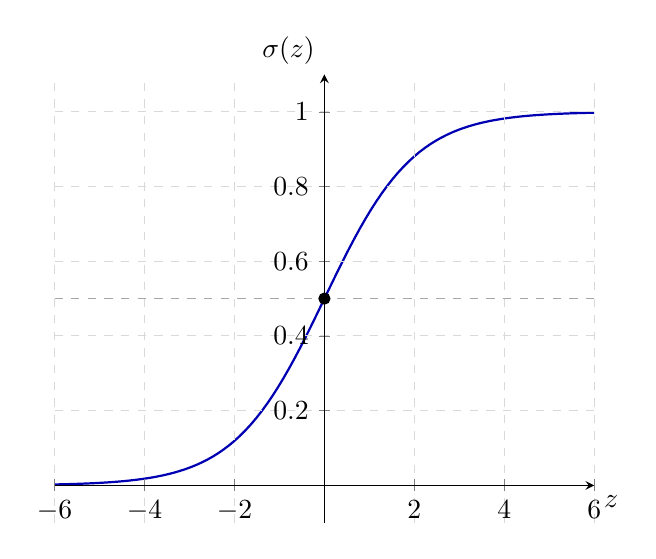
\begin{tikzpicture}
        \begin{axis}[
            xlabel={$z$},
            ylabel={$\sigma(z)$},
            xmin=-6.0, xmax=6.0,
            ymin=-0.1, ymax=1.1,
            axis lines=center,
            axis on top=true,
            grid=major,
            grid style={dashed, gray!30},
            every axis x label/.style={at={(current axis.right of origin)},anchor=north west},
            every axis y label/.style={at={(current axis.above origin)},anchor=south east}
        ]
            % Funzione Sigmoide: 1 / (1 + exp(-x))
            \addplot[domain=-6.0:6.0, samples=100, blue!70!black, thick] {1 / (1 + exp(-x))};

            % Linea orizzontale di asintoto a y = 0.5
            \draw[dashed, gray!70] (axis cs:-6.0,0.5) -- (axis cs:6.0,0.5);

            % Punto di flesso a (0, 0.5)
            \addplot[only marks, mark=*, black] coordinates {(0.0, 0.5)};

        \end{axis}
    \end{tikzpicture}
    \caption{Geometric representation of the sigmoid function.}
    \label{fig:sigmoid}
\end{figure}
The loss fuction is the \textbf{Binary Cross-Entropy Loss}:
\begin{equation}
    \mathcal{L}(y, \hat{y}) = -y \log \hat{y} - (1 - y) \log(1 - \hat{y})
\end{equation}
The model outputs a probability that the class is 1, so when z is large the loss is 
small; The smaller zeta becomes, the greater the loss becomes. For the class $y=0$ is mirrored. If 
we look at the formula \ref{formula:sigmoid}, the loss can't be really 0. 

\subsection{Multi-class Classification}
In multi-class classification tasks (e.g., Softmax Regression / Multinomial Logistic Regression), 
the model predicts a probability distribution across $C$ discrete classes. The output function is 
the \textbf{softmax} function, which maps a vector of raw scores 
$\mathbf{z} = [z_1, z_2, \dots, z_C]^T$ into a vector of probabilities $\hat{\mathbf{y}}$:
\begin{equation}
    \hat{y}_c = \text{softmax}(\mathbf{z})_c = \frac{e^{z_c}}{\sum_{j=1}^{C} e^{z_j}}
    \label{formula:softmax}
\end{equation}
where each predicted probability satisfies $\hat{y}_c \in (0, 1)$ and the sum of all probabilities 
equals one: $\sum_{c=1}^{C} \hat{y}_c = 1$. 
\newline
The loss function for multi-class classification is the \textbf{Cross-Entropy Loss}:
\begin{equation}
    \ell = - \log \hat{y}_y
\end{equation}
The softmax gives one probability per class ($\hat{y}_1, \dots, \hat{y}_k$) summing to 
1, and only the probability of the true class $y$ enters the loss.

\begin{figure}[H]
    \centering
    \begin{tikzpicture}
        \begin{axis}[
            xlabel={probability given to the true class, $\hat{y}_y$},
            ylabel={loss $\ell$},
            xmin=0.0, xmax=1.05,
            ymin=-0.5, ymax=4.5,
            axis lines=center,
            axis on top=true,
            grid=major,
            grid style={dashed, gray!30},
            every axis x label/.style={at={(current axis.right of origin)},anchor=north west},
            every axis y label/.style={at={(current axis.above origin)},anchor=south east}
        ]
            % Funzione Loss: -ln(x)
            \addplot[domain=0.02:1.0, samples=100, green!50!black, thick] {-ln(x)};

            % Punti specifici evidenziati
            \addplot[only marks, mark=*, black] coordinates {
                (0.1, 2.30)
                (0.5, 0.69)
                (0.9, 0.11)
            };

            % Etichette dei valori di loss in corrispondenza dei punti
            \node[above right] at (axis cs:0.1, 2.30) {\small $2.30$};
            \node[above right] at (axis cs:0.5, 0.69) {\small $0.69$};
            \node[above right] at (axis cs:0.9, 0.11) {\small $0.11$};

        \end{axis}
    \end{tikzpicture}
    \caption{Multi-class cross-entropy loss $\ell = -\log \hat{y}_y$ with specific examples.}
    \label{fig:multiclass_loss}
\end{figure}

\section{XOR Problem in Linear Model}
Models that rely purely on a linear score followed by a fixed non-linear output function 
(like logistic regression) are known as \textit{Generalized Linear Models}. Even though they apply 
a non-linear function (e.g., the S-shaped sigmoid curve), this function is strictly 
monotonic and only rescales the score. Consequently, the decision boundary,the region where the 
model decides to switch classes, remains a flat \textbf{hyperplane} ($z = 0$).
\newline
Consider the example in Fig \ref{fig:xor_problem}, suppose a linear
classifier $\hat{y} = 1$ $\iff$ $\mathbf{w}^{\top}\mathbf{x} + b \geq 0$. Now considering the four point
of the XOR:
\begin{itemize}
    \item (0,0): $b < 0$
    \item (1,0): $w_1 + b \geq 0$
    \item (0,1): $w_2 + b \geq 0$
    \item (1,1): $w_1 + w_2 + b < 0$
\end{itemize} 
we obtain the conditions for the parameters of the model, but if we combine the conditions for the intermediate
points: $w_1 + w_2 + b + b \geq 0 \implies w_1 + w_2 + b \geq -b$ but from the first condition we know
$b < 0$ so $w_1 + w_2 + b > 0$ but this is contradiction with the fourth condition. \textbf{No such w,b exists}.

\begin{figure}[H]
    \centering
    \begin{tikzpicture}
        \begin{axis}[
            xlabel={$x_1$},
            ylabel={$x_2$},
            xmin=-0.5, xmax=1.5,
            ymin=-0.5, ymax=1.5,
            axis lines=center,
            axis on top=true,
            grid=major,
            grid style={dashed, gray!30},
            xtick={0, 1},
            ytick={0, 1},
            every axis x label/.style={at={(current axis.right of origin)},anchor=north west},
            every axis y label/.style={at={(current axis.above origin)},anchor=south east}
        ]
            % Linee di collegamento del quadrato
            \draw[gray!40, thick] (axis cs:0,0) -- (axis cs:1,0) -- (axis cs:1,1) -- (axis cs:0,1) -- cycle;

            % Punti y = 1 (cerchi verdi)
            \addplot[only marks, mark=*, green!50!black, mark size=3.5pt] coordinates {
                (0, 1)
                (1, 0)
            };

            % Punti y = 0 (quadrati marroni/dorati)
            \addplot[only marks, mark=square, orange!60!black, thick, mark size=4pt] coordinates {
                (0, 0)
                (1, 1)
            };

            % Etichette dei punti
            \node[left, green!50!black, font=\small] at (axis cs:0, 1) {$y = 1$};
            \node[below, green!50!black, font=\small] at (axis cs:1, 0) {$y = 1$};
            \node[below left, orange!60!black, font=\small] at (axis cs:0, 0) {$y = 0$};
            \node[above right, orange!60!black, font=\small] at (axis cs:1, 1) {$y = 0$};

        \end{axis}
    \end{tikzpicture}
    \caption{Geometric representation of the XOR problem showing linear non-separability.}
    \label{fig:xor_problem}
\end{figure}
The only fix to solve those type of problem it is to compute the score on new features $\phi(x)$.
The \textbf{Representation} $\phi : \mathbb{R^d} \implies \mathbb{R^D}$, turns the d raw inputs into D
new features and then the model use those feature in the logit:
\[
f(\mathbf{x}; \theta, \mathbf{w}) = \phi(\mathbf{x}; \theta)^\top \mathbf{w} + b
\]
$\phi(x)$ can be obtained in three ways:
\begin{itemize}
    \item \textbf{Generic $\phi$}: a fixed rich map that poorly generalizes on hard problems
    \item \textbf{Hand designed $\phi$}: written by experts, expensive and demanding
    \item \textbf{Learned $\phi(\mathbf{x}; \theta)$}: learned by gradient descent
\end{itemize}